\documentclass[specification,annotation,times]{itmo-student-thesis}

%% Опции пакета:
%% - specification - если есть, генерируется задание, иначе не генерируется
%% - annotation - если есть, генерируется аннотация, иначе не генерируется
%% - times - делает все шрифтом Times New Roman, собирается с помощью xelatex
%% - pscyr - делает все шрифтом Times New Roman, требует пакета pscyr.

%% Делает запятую в формулах более интеллектуальной, например:
%% $1,5x$ будет читаться как полтора икса, а не один запятая пять иксов.
%% Однако если написать $1, 5x$, то все будет как прежде.
\usepackage{icomma}
\usepackage{tabularx}

%% Данные пакеты необязательны к использованию в бакалаврских/магистерских
%% Они нужны для иллюстративных целей
%% Начало
\usepackage{tikz}
\usetikzlibrary{arrows}
\usepackage{filecontents}
\begin{filecontents}{master-thesis.bib}
@incollection{ nsga-ii-steady-state,
    year        = {2009},
    booktitle   = {Nature-Inspired Algorithms for Optimisation},
    number      = {193},
    series      = {Studies in Computational Intelligence},
    title       = {On the Effect of Applying a Steady-State Selection Scheme in the Multi-Objective Genetic Algorithm {NSGA}-{II}},
    publisher   = {Springer Berlin Heidelberg},
    author      = {Nebro, Antonio J. and Durillo, Juan J.},
    pages       = {435-456},
    langid      = {english}
}


@inproceedings{ example-english,
    year        = {2015},
    booktitle   = {Proceedings of IEEE Congress on Evolutionary Computation},
    author      = {Maxim Buzdalov and Anatoly Shalyto},
    title       = {Hard Test Generation for Augmenting Path Maximum Flow 
                   Algorithms using Genetic Algorithms: Revisited},
    pages       = {2121-2128},
    langid      = {english}
}

@article{ example-russian,
    author      = {Максим Викторович Буздалов},
    title       = {Генерация тестов для олимпиадных задач по программированию 
                   с использованием генетических алгоритмов},
    journal     = {Научно-технический вестник {СПбГУ} {ИТМО}},
    number      = {2(72)},
    year        = {2011},
    pages       = {72-77},
    langid      = {russian}
}

@article{ unrestricted-jump-evco,
    author      = {Maxim Buzdalov and Benjamin Doerr and Mikhail Kever},
    title       = {The Unrestricted Black-Box Complexity of Jump Functions},
    journal     = {Evolutionary Computation},
    year        = {2016},
    note        = {Accepted for publication},
    langid      = {english}
}

@book{ bellman,
    author      = {R. E. Bellman},
    title       = {Dynamic Programming},
    address     = {Princeton, NJ},
    publisher   = {Princeton University Press},
    numpages    = {342},
    pagetotal   = {342},
    year        = {1957},
    langid      = {english}
}
\end{filecontents}
%% Конец

%% Указываем файл с библиографией.
\addbibresource{master-thesis.bib}

\begin{document}

\studygroup{Р42111}
\title{Алгоритмы определения размеров камней на видео на конвейере}
\author{Румянцева Мария Юрьевна}{Румянцева М.Ю.}
\supervisor{Балакшин Павел Валеревич}{Балакшин П.В.}{канд. техн. наук, доц.}{доцент Университета ИТМО}
\publishyear{2015}
%% Дата выдачи задания. Можно не указывать, тогда надо будет заполнить от руки.
\startdate{01}{сентября}{2013}
%% Срок сдачи студентом работы. Можно не указывать, тогда надо будет заполнить от руки.
\finishdate{31}{мая}{2015}
%% Дата защиты. Можно не указывать, тогда надо будет заполнить от руки.
\defencedate{15}{июня}{2015}

\addconsultant{Белашенков Н.Р.}{канд. физ.-мат. наук, без звания}
\addconsultant{Беззубик В.В.}{без степени, без звания}

\secretary{Павлова О.Н.}

%% Задание
%%% Техническое задание и исходные данные к работе
\technicalspec{Требуется разработать стилевой файл для системы \LaTeX, позволяющий оформлять бакалаврские работы и магистерские диссертации
на кафедре компьютерных технологий Университета ИТМО. Стилевой файл должен генерировать титульную страницу пояснительной записки,
задание, аннотацию и содержательную часть пояснительной записк. Первые три документа должны максимально близко соответствовать шаблонам документов,
принятым в настоящий момент на кафедре, в то время как содержательная часть должна максимально близко соответствовать ГОСТ~7.0.11-2011
на диссертацию.}

%%% Содержание выпускной квалификационной работы (перечень подлежащих разработке вопросов)
\plannedcontents{Пояснительная записка должна демонстрировать использование наиболее типичных конструкций, возникающих при составлении
пояснительной записки (перечисления, рисунки, таблицы, листинги, псевдокод), при этом должна быть составлена так, что демонстрируется
корректность работы стилевого файла. В частности, записка должна содержать не менее двух приложений (для демонстрации нумерации рисунков и таблиц
по приложениям согласно ГОСТ) и не менее десяти элементов нумерованного перечисления первого уровня вложенности (для демонстрации корректности
используемого при нумерации набора русских букв).}

%%% Исходные материалы и пособия 
\plannedsources{\begin{enumerate}
    \item ГОСТ~7.0.11-2011 <<Диссертация и автореферат диссертации>>;
    \item С.М. Львовский. Набор и верстка в системе \LaTeX;
    \item предыдущий комплект стилевых файлов, использовавшийся на кафедре компьютерных технологий.
\end{enumerate}}

%%% Календарный план
\addstage{Ознакомление с основами \LaTeX}{10.2014}
\addstage{Ознакомление с ГОСТ~7.0.11-2011}{10.2014}
\addstage{Ознакомление с имеющимся комплектом стилевых файлов и с кафедральными шаблонами документов}{12.2014}
\addstage{Реализация первоначальной версии стилевого файла}{02.2015}
\addstage{Написание пояснительной записки}{03.2015}
\addstage{Доработка стилевого файла и пояснительной записки}{05.2015}

%%% Цель исследования
\researchaim{Разработка удобного стилевого файла \LaTeX
             для бакалавров и магистров кафедры компьютерных технологий.}

%%% Задачи, решаемые в ВКР
\researchtargets{\begin{enumerate}
    \item соответствие титульной страницы, задания и аннотации шаблонам, принятым в настоящее время на
    кафедре;
    \item соответствие содержательной части пояснительной записки требованиям ГОСТ~7.0.11-2011 <<Диссертация и
    автореферат диссертации>>;
    \item относительное удобство в использовании~--- указание данных об авторе и научном руководителе один раз
    и в одном месте, автоматический подсчет числа тех или иных источников.
\end{enumerate}}

%%% Использование современных пакетов компьютерных программ и технологий
\advancedtechnologyusage{Была использована система компьютерной верстки \LaTeX, а в
рамках нее следующие пакеты, в порядке появления в стилевом файле: babel, csquotes,
geometry, amsmath, amssymb, amsthm,
amsfonts, amsextra, graphicx, xcolor, colortbl, tabu, caption, floatrow, algorithm,
algorithmicx, algpseudocode, enumitem, setspace, biblatex (а именно biber),
totcount, longtable, listings, chngcntr, titlesec, titletoc, ifpdf.}

%%% Краткая характеристика полученных результатов 
\researchsummary{Получился, надо сказать, практически неплохой стилевик. В 2015 году
его уже использовали некоторые бакалавры и магистры. Надеюсь на продолжение.}

%%% Гранты, полученные при выполнении работы 
\researchfunding{Автор разрабатывал этот стилевик исключительно за свой счет и на
добровольных началах. Однако значительная его часть была бы невозможна, если бы
автор не написал в свое время кандидатскую диссертацию в \LaTeX,
а также не отвечал за формирование кучи научно-технических отчетов по гранту,
известному как <<5-в-100>>, что происходило при государственной финансовой поддержке
ведущих университетов Российской Федерации (субсидия 074-U01).}

%%% Наличие публикаций и выступлений на конференциях по теме выпускной работы
\researchpublications{
\begin{refsection}
Однако покажу, как можно ссылаться на свои публикации из списка литературы:
\nocite{example-english, example-russian}
\printannobibliography
\end{refsection}
}

%% Эта команда генерирует титульный лист и аннотацию.
\maketitle{Магистр}

%% Оглавление
\tableofcontents

%% Макрос для введения. Совместим со старым стилевиком.
\startprefacepage
Настоящая работа посвящена исследованивания для автоматизации рудоподготовки, а именно применения компьютерного зрения для построения распределения камней руды на конвейере для управления дробилкой.

В настоящее время управление дробилкой для камней камней осуществляется вручную. Реализованный программный продукт поможет автоматизировать процесс управления дроблением камней - при нахождении на конвейере большого количества крупных камней необходимо убыстрять дробилку, при большом количестве мелких камней - замедлять. 

%˗ решаемую проблему;

В настоящий момент в основном управление мельницей реализовано за счёт визуальной  оценки  человек распределения камней по размеру. \textit{Проблема} использованного метода заключается в том, что данная оценка является неточной и субъективной, так как человеку сложно оценить реальное соотношение больших, средних и маленьких камней руды. \textit{Решением} проблемы является проведение визиометрического анализа с помощью компьютерного зрения.

В качестве входных данных используется видео движения конвейера, на котором находятся камни руды. Необходимо детектировать камни на ленте и рассчитывать их размер, а также  отслеживать их перемещение, чтобы выполнить построение распределения объектов по размеру и определить скорость дробилки. Отслеживание перемещения используется для гарантии построения верного распределения. 

%˗ цели и задачи;
	
\textit{Целью} данной работы является выбор подходящего алгоритма или сочетания алгоритмов для распознавания и построения распределения камней с дальнейшим построением распределения камней по конвейеру для дальнейшей разработки программного обеспечения для автоматизации дробилки. \textit{Объект исследования} - автоматизация рудоподготовки, предмет исследования - применения компьютерного зрения для детектирования и отслеживания камней на конвейере. 

Компьютерное зрение успешно применяется для распознавания объектов на видео. Решение задачи, основанное на компьютерном зрении, состоит из следующих шагов: предварительная обработка кадра изображения, детектирование камней на ленте, оценка размеров, построение распределение, отслеживание на следующем кадре.
Первый шаг - предварительная обработка кадра изображения, цель обработки - повысить качество изображения, которое позволит однозначно определить объекты камней на ленте. Второй шаг - детектирование камней с целью получить координаты камней на видео. Необходимо детектировать как можно большее количество как крупных, так и мелких камней. Третий шаг - построение распределение камней по размеру для формирования скорости для дробилки. Четвертым шагом является отслеживание камней с целью соотнести уже определённые камни с объектами. 

Таким образом, для проведения исследования нужно решить следующие задачи:
\begin{enumerate}
	\item Разработать методы и программные средства для предварительной обработки кадров ленты конвейера
	\item Разработать методы и программные средства для детектирования камней на ленте
	\item Разработать методы и программные средства для отслеживания камней на видео
	\item Разработать методы и программные средства для построения распределения
\end{enumerate}

Далее мы рассмотрим мотивацию исследования и обзор существующих решений

%- актуальность темы исследования;


%˗ степень ее разработанности;




%˗ практическую значимость работы.
%˗ научную новизну;
%˗ методы исследования;
%˗ методологическую и теоретическую основы исследования;
%˗ положения, выносимые на защиту;
%˗ степень достоверности и апробацию результатов.
%% Начало содержательной части.
\chapter{Анализ предметной области}
В данной главе рассматривается основа исследования из области автоматизации процессом производства металлов, проводится обзор существующих решений для автоматизации управления мельницей для дробления. Приводится обзор основных методик компьютерного зрения.
%% Так помечается начало обзора.
\startrelatedwork
\section{Введение в рудоподготовку}
Существует ряд горно-металлургических компаний, производящих различные металлы. Одним из таких предприятий является компания <<Норникель>>, производящая рафинированный никель, палладий и другие ценные металлы. Компания <<Норникель>> -- лидер горно-металлургической отрасли России и   крупнейший в мире производителем высокосортного никеля и палладия. 

\subsection{Процесс рудоподготовки}
Для производства ценных металлов необходима добыча руды. Руда проходит дальнейшую рудоподготовку для того, чтобы из неё можно было выделить металлы. 

\textit{Рудоподготовка } --- совокупность процессов и технологий обработки руды различными методами с целью определить гранулометрический и вещественный состав для последующего использования. Технологическая схема обработки сырья  зависит от назначения итогового продукта. 

Рудоподготовка включает в себя следующие процессы: 
\begin{itemize}
\item дробление;
\item грохочение;
\item измельчение;
\item классификация;
\item агломерация (окускование);
\item шихтование.
\end{itemize}

\textit{Дробление} - процесс разрушения руды или любого другого материала с целью получения материала необходимного гранулометрического состава размером куска более 5 мм. Дробление основано на действии внешних сил, чаще всего применяется механическое дробление. По крупности результирующего продукта выделяют крупное (100-350 мм), среднее (40-100 мм), мелкое дробление (5-40 мм).  Измельчение - достижение кусков руды размеров менее 5 мм (следующая стадия за дроблением).

Часто перед дроблением призоводят \textit{грохочение} - исходный материал поступает на грохот - устройство с калиброванными отверстиями или щелями для сортировки сыпучих материалов по крупности частиц. Грохочение позволяет убрать камни, дробление которых не предусматривается этим этапом обработки.

Процесс \textit{классификации} - разделение измельчённых элемнте на основе различий в скоростях оседания частиц разного размера и плотности с целью получения продукта разного гранулометрического состава. Процессу классификации подвергается продукта крупностью менее 3 мм.

Агломерация - процесс укрупнения измельченных камней руды для подготовки к последующему переделу. Шихтование - смешивание сырья разных сортов для придание смеси определённых свойств.

Нас в первую очередь интересует процесс дробления и предшествующий ему процесс определения гранулометрического состава.
\subsection{Гранулометрический состав}
\textit{Гранулометрический состав} (granulometric соmposition) -- распределение камней руды по крупности, характеризующееся процентным выходом от массы или количества кусков руды. 
Гранулометрический состав - важный физический показатель качества руды.  Состав сырья влияет на дальнейшее дробление и измельчение, а так же на вариативность использования. Определением гранулометрического состава занимается \textit{гранулометрия}.

В горнодобывающей отрасли размер частиц влияет на очень  много процессов, включая подрывание, дробление и окускование. В результате значительные усилия прилагаются к измерению или оценке распределения частиц по размерам, чтобы оценить и оптимизировать производство с точки зрения производительности и затрат на производство (затраты на энергию, материалы и оборудование). Операторы шахт и карьеров хотят измерить результаты определения размера частиц всех этих видов деятельности, но просеивание / сортировка является несовершенным инструментом оценки из-за медленной обратной связи и непоследовательных измерений из-за усталости оператора или изменений в технике. В результате появилась возможность создания онлайновых бесконтактных, полностью автоматизированных систем машинного зрения для измерения размера частиц, что облегчает оценку и оптимизацию процессов добычи и обработки частиц.
От качества определения гранулометрического состава зависит дальнейшее качество обработки.


\section{Обзор существующих решений}
Существует ряд различных подходов к гранулометрии руды. 

 Стандартом для оценки распределения частиц является ситовой аналищ,  применяемый к забору пробы руды из контейнера (около 1$m^3$). Механическое просеивание используется для разделения частиц на ситовые фракции с анализом, основанным на принципе того, что размеры частиц могут быть оценены с использованием ситовых рам разных размеров.  Данный метод позволяет обходиться без дополнительных устройств. Забор руды проиходит несколько раз в сутки. Точность этого метода достаточно низкая, так как он работает на допущении, что камни распределены по контейнеру равномерно, и в любой порции камней распределение будет одинаково, что вероятнее всего приведёт к низкой эффективности работы мельницы. Такой подход всё ещё применяется на некоторых предприятиях. 
 
Ручный или визуальный гранулометрический анализ является неточным, поэтому естественно желание компаний автоматизировать процесс. Существует ряд высотехнологических решений, основанных на различных подходах, реализованными компаниями. Далее приведём краткий обзор технологических решений компаний в таблице ~\ref{tab1}.
 
 Одним из технологий проведения гранулометрического анализа является  сочетание инфракрасной трехмерной съемки и различных алгоритмов обработки изображений. Таким образом проводит анализ анализаторы <<SizeScan>>.  Методика инфракрасной съемки в невидимом человеческому глазу спектре разработана компанией <<COREM>>. Для съемки используются специальные  трехмерные камеры,  которые позволяют осуществлять анализ объёмного изображения. 
 
 Анализатор <<Outotec RockSense>> осуществляет гранулометрию с помощью трехмерного лазерного сканирования, а не инфракрасной съёмки. На основе данных сканирования формируется объёмное изображение.
 
Ряд устройств работает  с помощью флуоресцентного рентгенорадиометрического метода, например  .  В основе этого метода лежит зависимость плотности потока характеристического рентгеновского излучения химических элементов от их концентраций.
Минусом данных промышленных подходов является дорогостоящее специализированное оборудование для съёмок. 

\begin{table}[!h]
	\caption{Обзор промышленных решений по автоматизации гранулометрии}\label{tab1}
	\centering
	\begin{tabularx}{\textwidth}{|*{7}{>{\centering\arraybackslash}X|}}\hline
		Авторы  & Подход &Реальное время & Ручная корректировка& Точность \\\hline
		Конвелс &  CV & да 	& нет & до 99\% \\\hline
		Madrobots DL & CV, ML & нет  & нет& 80\% \\\hline
		ООО «Техноаналитприбор» & РФА  & да & нет & н.д. \\\hline
		SizeScan  & 3D сканирование & да & нет & - \\\hline
		Outotec RockSense & лазерное сканирование   & да & нет & - \\\hline
		Split Desktop & классический CV & нет & нет & -\\\hline
	\end{tabularx}
\end{table}
Существующие промышленные решения являются пропиетарными и конкретных данных о деталях реализации и точности не приводится.
Продукты для грануляционного анализа конфигурируются для конкретного производства из-за отличаюшихся условия, такие как размер ленты конвейера, освещенность, возможностью установки технических устройств, состав продукта. Чаще всего предприятиям предлагается готовый аппаратно-программный комплекс, сконфигурированный под конкретное предприятие.

Проблема автоматизация определения гранулометрического состава стоит давно, и попытки решить её с использованием компьютерного зрения и анализа изображений были предприняты ещё в 1980-х годах. 
Приведём краткий обзор исследовательских работ по проведению гранулометрии с использованием компьютерного зрения в таблице \ref{tab2}.

\begin{table}[!h]
	\caption{Обзор исследований по автоматизации гранулометрии}\label{tab2}
	\centering
	\begin{tabularx}{\textwidth}{|*{7}{>{\centering\arraybackslash}X|}}\hline
		Автор  & Год& Подход& Реальное время & Ручная корректировка& Точность \\\hline
		Молдован Д.В.	& 2006 & классические методы CV & нет & да 	& - \\\hline
		Andersson T & 2010 & 3D карта изображения, класс. CV & да & нет  &  \\\hline
		Хурэлчулуун И. & 2019 & классические методы CV & да & нет & 89\%  \\\hline
		E.Hamzeloo et al &  2014 & CV, PCA-NN &  нет & нет & -	\\\hline
		S. Al-Thyabat et al & 2006 & классические методы CV & нет  & нет  & 78\%\\\hline
		Matthew J Thurley & 2014 & 3D карта изображения, класс. CV & да & нет  & \\\hline
	\end{tabularx}
\end{table}


Исследования используют в качестве базы как двухмерные изображения, так и трёхмерные. Большая часть исследований посвящена двумерным изображением, что, вероятно, обусловлена технологической доступности установки обычных камер на производстве и сложность установки устройств, позволяющих получить 3D-картину, таких как лазерный сканер или 3D-камера. К сожалению, данные исследований в основном не содержат численных данных о точности оценки, поэтому можно орентироваться лишь на визуальные данные.

Чаще всего в качестве методов анализа изображения исследователями используются классические методы компьютерного зрения, основанные на математических преобразования изображений. Первым этапом во всех исследованиях является предобработка изображений, целью которой является качественная бинаризация. Часть исследований считает удовлетворительным результат бинаризации или простого выделения контуров в качестве для выделения отдельных камней (Split desktop). Некоторые исследования применяют машинное обучение и нейронные сети.

Интерес к автоматизации управления мельницами на производстве до сих пор высок, о чём свидетельствуют наличие исследований последних лет. Развитие методов машинного обучения позволяет вывести качество анализа на новый уровень. 


\subsection{Проблемы определния камней на ленте конвейера}

При сегментации камней могут возникнуть ряд проблем, снижающих точность анализа. Причиной этих проблем является то, что фотографические методы измеряют только то, что видно на поверхности кучи на конвейере, и необходимо учесть эти ошибки для гарантии того, что измерения будет стабильным и надежным. Рассмотрим ключевые ошибки.

\textit{Ошибка разграничения частиц} является неточностью определения правильного разделения отдельных частиц на измеряемой поверхности. Мелкие частицы для алгоритма компьютерного зрения могут являются одной большой частиц. 

Ошибка частиц субразрешения связана с неспособностью системы анализа видеть мелкие частицы ниже разрешения сенсора. Эти частицы субразрешения имеют тенденцию группироваться в более крупные области и могут иметь неправильный размер в виде крупных камней.

\textit{Эффект бразильского ореха} - ошибка сегрегации и группировки, которая описывает тенденцию кучи разделяться на группы фрагментов одинакового размера, вызванных вибрацией или движением кучи камня, например при движении грузовика или на конвейерные ленты.

Методы анализа поверхности, основанные на компьютерном ззрении, чувствительны к ошибкам сегрегации и группировки и могут привести к большим ошибкам выборки, если цель состоит в том, чтобы вычислить распределение по размеру для всей кучи. 

Существуют три возможности для минимизации этой ошибки. Первое решение состоит в том, чтобы разместить камеру непосредственно после некоторого гомогенизирующего оборудования. Однако установка гомогенизирующего оборудования может быть непрактичной для существующих установок, так как это потребует модернизации систем конвейерной ленты. Это решение подходит только для заводов, которые будут построены в будущем. Второе решение заключается в разработке моделей, которые могут описывать динамику в куче частиц, когда частицы транспортируются на конвейерные ленты; однако моделирование динамики кучи является сложной задачей. Наиболее практичным решением для минимизации ошибок сегрегации и группировки является размещение оборудования для отбора проб в месте, где существует ограниченная ошибка сегрегации и группировки. Например, непосредственно после дробилок для обломков породы.

\textit{Ошибка перекрывающихся частиц} вызывает отклонение измерение в сторону увеличения количества камней меньших размеров, так как перекрытые области камней рассматриваются как мелкие неперекрытые камни. Эту ошибку можно преодолеть в кучах сыпучего материала, если использовать данные трехмерного сканирования. Согласно исследованиям, это обеспечвает  точность около 82\% классификации камней по размеру.

\textit{Ошибка профиля} описывает возможную ошибку, возникающую из-за того,  что видна только одна сторона (профиль) неперекрытого камня что затрудняет оценку размера камней. Данная ошибка определяется в первую очередь на двумерных изображениях.

\textit{Разграничение и извлечение образца} - ошибка, относящаяся всем методам отбора проб с конвейера из-за неправильного определения границ секции конвейера при использовании двух параллельных срезов по всей длине ремня. Частью образца являются только частицы, центр тяжести которых находится внутри области, ограниченной срезами.

\section{Мотивация исследования}
Сейчас на рудообрабатывающих предприятиях компании <<Норникель>> выставление скорости дробления вручную на основе визуальной субъективной оценки. Скорость работы дробилки зависит от того, какого размера камни видит мастер, следящий за лентой конвейера. 

Данный подход является затратным, так как необходимо иметь сотрудника, который будет осуществлять визуальный анализ, и может привести к ошибкам определения, так как человек определяет степень распределения камней без каких-либо измерений субъективно, что не позволяет достичь максимальной энергоэффективности в управлении дробилкой. Так же подход не позволяет стандартизировать процесс производства, что ограничивает качество финальной продукции.

Задачей оптимизации управление мельницы является сохранение максимальной загрузки при качественном измельчении. 

Автоматизация гранулометрии позволит повысить точность управления дробилкой руды. В настоящий момент работа мельницы не максимально эффективна, так как крупных камни перемалываются дольше медленных, и возможна ситуация, когда при большом количестве крупных камней мельница не успеет обработать всё сырье, или наоборот, перемолоть быстро, но некачественно. При автоматизации с использованием компьютерного зрения эти проблемы не будут возникать. 

Использование компьютерного зрения при решении задачи автоматизации гранулометрии является наиболее дешёвым из высокотехнологических методов, так как требует только видеокамеры и осветительных приборов, которые уже установлены. Использование уже существующих решений неэффективно, так как требует установки своего оборудования взамен уже существующего.


Существуюшие решения для проведение гранулометрического анализа с использованием компьютерного зрения используют  как простые классические, так и методы компьютерного зрения с использованием машинного обучения. Использование машинного обучения требует  аппаратных ресурсов для проведения вычисления. Так же не исследовалась возможность отслеживать изменения распределения камней с использованием детектирования - все существующие решения основаны только на постоянной сегментации и перерасчёте распределения.

В данной работе предполагается исследовать возможность использования отслеживания перемещения камней по конвейеру для уточнения построения распределения камней и оптимизации вычисления. Так же предполагается исследовать использования методов оптического потока для построения распределения.


\section{Обзор методов компьютерного зрения}
\textit{Компьютерное зрение}, часто используют аббревиатуру CV — направление исследований в области искусственного интеллекта и связанные с ним технологии получения изображений объектов реального мира, их обработки и использования полученных данных для решения разного рода прикладных задач без участия (полного или частичного) человека. Другими словами, компьютерное зрение - область ислледований, помогающих компьютерам "видеть" как человек. На абстрактном уровне, проблематика компьютерного зрения - использование данных с наблюдаемого изображения для того, чтобы сделать вывод о мире. Интенсивное изучение этой отрасли началось с 1970-х годов.

Связанной отраслью является машинное зрение  - область применения компьютерного зрения для решения промышленных задач.  Компьютерное зрение представляет собой общий набор методов и алгоритмов, позволяющих компьютерам производить анализ изображений, тогда как машинное зрение комбинирует применение компьютерного зрения с системами ввода-вывода, компьютерными сетями и прочим.  Системы машинного зрения решают более узкоспециализированные задачи, чем компьютерное зрение, например, распознавание автомобильных номеров или определение скорости автомобиля. В данной работе мы сфокусируемся на применении алгоритмов компьютерного зрения.

Обработка изображений не является предметов компьютерного зрения, но часто используется для подготовки необработанных данных. Иными словами, перед анализом изображения часто производят предобработку (препроцессинг).

Методы компьютерного зрения часто разделяют на классические (с помощью математических преобразований изображений) и с использованием машинного обучения.  


\subsection{Задачи компьютерного зрения}\label{cvtasks}
Существует ряд задач, традиционно относимых к компьютерному зрению и решаемых с помощью него:
\begin{itemize}
\item распознавание;
\item распознавание текста;
\item детектирование;
\item идентификация;
\item восстановление сцены;
\item восстановление изображений;
\item сегментация изображений;
\item отслеживание;
\item анализ оптического потока.
\end{itemize}

\textit{Распознавание} - одна из  классических задача компьютерного зрения. Распознование объектов - определение, содержит ли фотография или видео определённый объект. Задача легко решается человеком, но до сих пор не решена в общем случае для компьютера для случайных объектов в случайном окружении. 


\textit{Распознавание текста} -поиск и распознавание символов на изображении - как печатных, так и рукописных. 

\textit{Идентификация} - распознавание экземпляра определённого класса объекта на основе признаков, например идентификация определённого человека по лицу или по отпечатку пальца.

\textit{Детектирование} - проверка входных данных на наличие определённого класса объектов. 

Лучше всего для решения данных задач подходят свёрточных нейронные сети. Производительность решений, основанных на нейронных сетях, сейчас близка к человеческой. 

\textit{Восстановление сцены } - задача построения сцены по данным нескольких двумерных изображений или по видео. В простейшем случае мы получаем набор точек, описывающих сцену, в более сложных случаях возможно получить полную трёхмерную модель поверхности. 

\textit{Восстановление изображений} - задача, направленая на улучшение качества фотографий - удаление шума или повышение чёткости объекта. В последнее время становятся популярными алгоритмы, позволяющие с помощью нейронных сетей раскрасить чёрно-белую фотографию или перевести в формат высокий чёткости.

\textit{Сегментация изображений} - разбиение изображение на множество областей по каким-либо признакам. Сегментация позволяет отделить объекты изображения друг от друга. 

\textit{Отслеживание } - задача, направленная на определение нового положения уже определённого ранее объекта на видео. Примером отслеживания  может служит определение движущейся машины ны фотографии.
\textit{Оптический поток} определяется как видимое движение отдельных пикселей на плоскости изображения. Часто векторы движения, полученные при вычисление оптического потока являются хорошим приближение к истинному физическому движению, спроецированному на плоскость.

В данной работе целесообразно исследование различных методов распознавания, сегментации,отслеживания и анализа оптического потока для решения поставленной задачи, как соотносящихся с традиционными методами решения схожих проблем. Конкретные методы будут рассмотрены более подробно в главах 2, 3 и 4.
\subsection{Методы компьютерного зрения}\label{cvmethods}

Конкретная реализация системы компьютерного зрения сильно зависит от задачи, которая эта система решает. Некоторые системы являются автономными приложениями, решающие специфическую проблему анализа или детектирования, в то же время, другие являются частями более крупных систем, включающими так же модули для управления механизмами, модули баз данных, человек-компьютерные интерфейсы.
Многие методы являются уникальными для системы, однако существуют типичные методы, которые используются в большинстве системах компьютерного зрения.


\textit{Получение изображения} - цифровое изображение создаётся из результатов работы одного или нескольких датчиков изображение, в роли которых может быть светочувствительная камера, 3D-камера, лидар и т.д.  В зависимости от типа датчика, результирующее изображение может представлять  двухмерное или трехмерное изображение или совокупность изображений. Значения пикселей обычно соответствуют интенсивности света в одной или нескольких спектральных полосах (изображения в оттенках серого или цветные изображения), но также могут быть связаны с различными физическими измерениями. 

\textit{Предварительная обработка} - чаще всего перед извлечением данных из изображения, его необходимо подготовить, чтобы убедиться, что оно удовлетворяет условиям, подразумевающихся используемым методом, а так же облегчить извлечение данных. Например:
\begin{itemize}
	\item  Снижение уровня шума для гарантии отсутствия ложных данных.
	\item Повышение уровня констрастности для гарантии, что интересующие нас данные могут быть извлечены.
	\item Масштабирование, поворот.
\end{itemize}

\textit{Извлечение признаков }-  на этом этапе из изображения извлекаются признаки, описывающие изображение. 
Типичные примеры таких признаков:
\begin{itemize}
	\item  Линии, края и границы.
	\item Локализованные маркеры, такие как углы или точки.
	\item Более сложные признаки, получаемые из текстуры или формы. 
\end{itemize}

\textit{Обнаружение / сегментация} - в процессе обработки принимается решение о том, какие области изображения необходимы для дальнейшего анализа. Например:
\begin{itemize}
	\item  Выделение набора точек интереса.
	\item Сегментация областей изображения, содержащих интересующий нас объект.
	\item Выделение объектов первого плана, создание иерархии сцен
\end{itemize}

\textit{Высокоуровневания обработка} - на этом этапе извлеченные данные пригодны соотвествуют какому-либо объекту и мы можем принять решение, решая одну из задач, описанных  в пункте \ref{cvtasks}.

Решение задачи гранулометрии требует 
\subsection{Методы обработки изображений}
Предобработка изображений, как уже было сказано в пункте \ref{cvmethods}, используется для подготовки изображения к извлечению данных.
Выделяют следующие основные методы обработки изображений:

\begin{itemize}
	\item \textit{Фильтры}, с помощью которых проивзодится размытие изображения или повышения резкости. Наиболее частое применение фильтров - избравление от шумов.  Так же с помощью фильтров возможно выделение краёв объекта. 
	\item \textit{Афинные преобразования}, такие как поворот, масштабирование или изменения соотношения сторон.
	\item Морфологические преобразования, такие как размыкание и замыкание. Преобразования помогают выделить конкретные объекты переднего плана.
	\item Бинаризация - приведение изображения в двоичный вид.
	\item Работа с гистограммой - например, эквализация, позволяющая повысить яркость изображения.
\end{itemize}
Более подробно алгоритмы данных методов и их применение будут рассмотрены в следующих главах.

\chapterconclusion


\chapter{Алгоритмы детектирования объектов}
В данной главе описываются методы детектирования объектов на кадрах видео. Расматриваются
алгоритм поиска контуров на основе топологического структурного анализа оцифрованных двоичных изображений по границе, алгоритм максимально стабильных экстремальных областей, детектор границ Кенни, оператор Собеля. Так же рассматривается использование метода маркерного водораздела. 

\section{Набор данных}
В качестве исходных данных используется видео с камеры конвейера на предприятии <<Норникель>> (рис. \ref{fig:lenta}). Камера установлена над конвейером и захватывает небольшой участок. 
Изображение содержит ленту с находящимися на ней камнями и небольшие участки окружающей среды.
\begin{figure}[h!]
	\centering
	\includegraphics[width=0.8\linewidth]{images/lenta}
	\caption{Лента конвейере с рудой}
	\label{fig:lenta}
\end{figure}

В качестве исходных данных используется видео записи конвейера длиной 5 минут. Исходное видео требует предобработки, так как в кадре находится не только конвейер, но и окружающая среда, а так же оно низкоконтрастное. 

Сложность выделения отдельных камней на конвейере определяется тем, что камни представляют собой однородные объекты без чётких признаков, по которым их можно отделить от других объектов. Так же видно потенциальную ошибку разграничения частиц - мелкие частицы представляют собой единый поток, который для алгоритма компьютерного зрения может представлять один большой камень. Тем не менее, средние и большие камни достаточно чётко различимы на фоне конвейера.


\section{Предварительная обработка изображений}
Цель предобработки изображений - подготовить исходные данные изображения для извлечения необходимой нам информации, повысить вероятность определения именно тех объектов, которые нам необходимы.

Исходные кадры с конвейера требуют предобработки, так как имеют низкую яркость, и объекты сложно различимы. Дополнительную сложность вносит однородность объектов. Задача предобработки - выделить объекты для дальнейшего анализа.

Предварительная обработка изображения (кадра видео) включает в себя:
\begin{enumerate}
	\item Кадрирование изображения для выделения ленты конвейера. Кадрирование является наиболее простым шагов предобработки и позволяет не выявить лишних деталей.
	\item Уменьшение шума путём применения размытия по Гауссу. Фильтр Гаусса часто применяется для сглаживания изображения, но  так же часто его применение для удаления шумов и улучшения структуры  изображения. Гаусовская фильтрация является результатом применения функции Гаусса к каждому пикселю изображения, иными словами, фильтр осуществляет свёртку каждого пикселя, вычисляя среднее значение на основе всех точек, находящихся в определённом радусе изображения (размер окна).
	\item Эквализация гистограммы. Данная операция позволяет повысить яркость и контраст изображения. Цель эквализации - преобразование гистограммы таким образом, чтобы она соответствала нормальному закону распределения. Эквализация гистограммы происходит следующим образом: вычисление гистограммы исходного изображения (так как исходное изображение должно быть 8-битным одноканальным изображением, то в данном случае взят канал значение (Vue) цветовой модели HSV), после этого гистограмма нормализуется путём деления значения каждого бина гистограммы на общее количество пикселей, вычисление интегральной функции распределения на основе исходного изображения и вычисление нового значения интесивности каждого пикселя на основе этой функции.
	\item Сокращение количества цветов изображения для увеличения скорости дальнейшего анализа.
\end{enumerate}

Алгоритмы, которые мы будем использовать в дальнейшем, использую в качестве входных данных изображение в оттенках серого, так что последним этапов будет преобразование изображения к оттенкам серого. 

Результаты каждого этапа предобработки можно видеть на рисунке \ref{fig:preprocessing}. Исходный код функции предобработки представлен в листинге \ref{lst:preprocessings}.
\begin{figure}[h!]
	\centering
	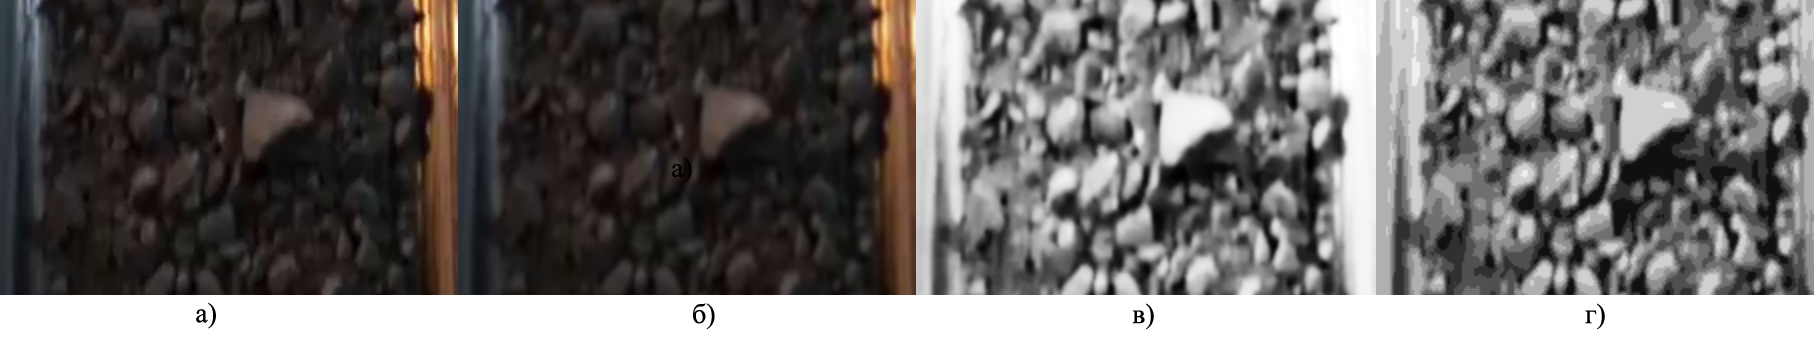
\includegraphics[width=\linewidth]{images/preprocessing}
	\caption{Процесс предобработки изображения: а) исходное изображение, б) изображение после размытие, в) после эквализации гистограммы, г) после уменьшения количества цветов }
	\label{fig:preprocessing}
\end{figure}

\begin{algorithm}[!h]
	\caption{Исходный код функции преобработки:}\label{lst:preprocessing}
	\begin{lstlisting}
	def preprocessing(frame):
	frame = frame[0:700, 130:360]
	cv2_imshow(frame)
	frame = cv2.GaussianBlur(frame,(3,3),0)
	hsv = cv2.cvtColor(frame, cv2.COLOR_BGR2HSV)
	h, s, v = cv2.split(hsv)
	v = cv2.equalizeHist(v)
	hsv = cv2.merge([h, s, v])
	bgr = cv2.cvtColor(hsv, cv2.COLOR_HSV2BGR)
	gray = cv2.cvtColor(bgr, cv2.COLOR_BGR2GRAY)
	div = 32
	gray = gray // div * div + div // 2
	
	return bgr, gray
	\end{lstlisting}
\end{algorithm}

Результатом работы данного этапа является обработанное изображение с повышенной яркостью и уменьшенными шумами. На полученном изображении объекты чётко выделяются на фоне.


\section{Детектирование камней}
Несмотря на то, что технически рассмотренные ниже методы являются методами извлечения признаков и сегментации, но в условиях задачи определения камней уместно называть их методами детектирования камней. Рассмотрим базовые методы определения границ объектов. 
\subsection{Алгоритм следования границ}
Стандартным методом определения контуров является метод следования границ (border following). В библиотеке OpenCV именно этот алгоритм реализует функция \texttt{findContour()}. Данный алгоритм чаще всего применяется на бинаризованных изображениях и определяет внешние и внутренние границы контуров объектов путём обхода изображений, находя продолжение контура среди соседей текущего пикселя. Алгоритм позволяет определить иерархию контуров изображения - внешних и внутренних, внутренним контуром считается контур, находящийся внутри другого контура. 

\begin{figure}[h]
	\centering
	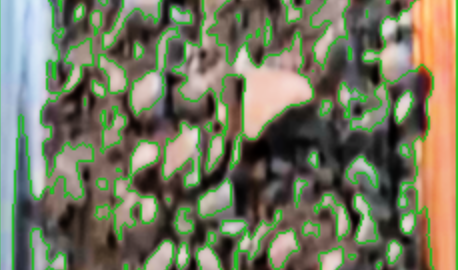
\includegraphics[width=0.7\linewidth]{images/findContour}
	\caption{Результат применения алгоритма следования }
	\label{fig:findcontour}
\end{figure}


В качестве входных данных необходимо использовать 8-битное одноканальное изображение.
Результат применения данного алгоритма к ленте конвейера (рис. \ref{fig:findcontour}) является удовлетворительным, так как алгоритм смог выделить светлые области на изображении, часто совпадающие с камнями, но однако мы можем наблюдать ошибку профиля (рис. \ref{ris:findContours}a) и ошибку разграничения частиц (рис. \ref{ris:findContours}б)

\begin{figure}[h]
	\begin{minipage}[h]{0.49\linewidth}
		\centering
			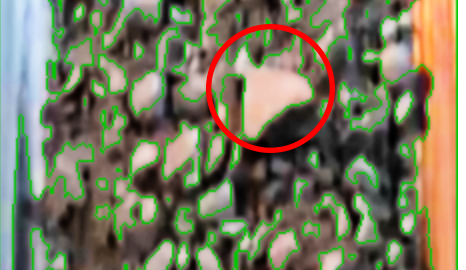
\includegraphics[width=0.9\linewidth]{images/findContour_profile} \\ a)
	\end{minipage}
	\hfill
	\begin{minipage}[h]{0.49\linewidth}
		\centering
		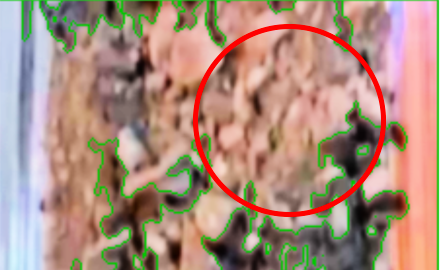
\includegraphics[width=0.9\linewidth]{images/findContours_sep} \\ б)
	\end{minipage}
	\caption{Ошибки, возникшие при применении алгоритма следования границам.}
	\label{ris:findContours}
\end{figure}



\subsection{MSER}
Алгоритм MSER отличается от алгоритма поиска контуров тем, что он ищет схожие области на основе  экстремального свойством функции интенсивности в области и на ее внешней границе, а не границы изображения. Использование  данного алгоритма осуществляется с помощью класса MSER и метода detectRegions[9], принимающего как единственный параметр значения изображения
\subsection{Детектор границ Кенни}
\subsection{Оператор Собеля}
\subsection{Метод водораздела}
Простые методы не могут выделить 
\subsubsection{Вычисление маркеров}
\subsubsection{Вычисление регионов}

\chapterconclusion


\chapter{Алгоритмы отслеживания объектов}
В качестве алгоритмов отслеживания были выбраны:

Алгоритм  Multiple Instance Learning (MIL) [4], как имеющий хорошую точность[5], в качестве основы выбран класс OpenCV Multitracker. Алгоритм MIL обучает классификатор в режиме онлайн, чтобы отделить объект от фона. MIL обозначение обучение нескольких экземпляров позволяет избежать проблемы смещения для надежного отслеживания.

Корреляционный трекер библиотеки dlib. Реализация этого алгоритма базируется на алгоритме MOSSE (Minimum Output Sum of Squared Error Filter), предлагает использовать масштабную пирамиду, чтобы точно оценить масштаб объекта после того, как было найдено оптимальное отражение. 

Комбинация корреляционного и центроидного трекеров (корреляционный трекер dlib + самостоятельная реализация). Центроидный трекер  используется в дополнение к корреляционному. Он принимает начальные координаты прямоугольника, описывающего объекты и формирует объект центроида. Каждому центроиду присваивается новый идентификатор. После обновления кадра вычисляется евклидово расстояние между новыми ограничительными рамками и существующими объектами, и на основе минимального расстояния объектам присваиваются старые или новые идентификаторы.

\section{Методы OpenCV для отслеживания объектов}
\section{MIL}
Для использования данного алгоритма необходимо создать контейнер для трекеров. В данном случае в качестве контейнера используется экземпляр класса OpenCV MultiTracker.
Для отслеживания изображения необходимо инициализировать трекеры: детектировать объекты одним из подходящих способов, после этого для каждого из детектированных объектов создать экземпляр класса cv2.TrackerMIL с помощью метода cv2.TrackerMIL\_create и добавить в лист трекеров. При каждой смене кадра необходимо вызвать метод update()  листа трекеров для обновления списка координат. 
Результатом работы данной программы является отслеживание движения камней по конвейеру.


Были выявлены следующие положительные стороны:
высокая точность отслеживания;
автоматическое очищение треков при пропадании из кадра.
Были выявлены следующие проблемы:
снижение скорости из-за накопления трекеров;
необходимость запускать детектирование новых объектов;
сброс существующих трекеров при детектировании новых.

\section{Корреляционный трекер}
Для использования данного алгоритма так же необходимо создать контейнер для трекеров. В данном случае в качестве контейнера используется экземпляр класса OpenCV MultiTracker.
Для отслеживания изображения необходимо инициализировать трекеры: детектировать объекты одним из подходящих способов, после этого для каждого из детектированных объектов создать трекер с помощью метода dlib.correlation\_tracker(), а так же задания объект для отслеживания с помощью метода dlib.rectangle(), принимающего как параметр значения координат углов окружающего объект прямоугольника, после этого начать отслеживание с помощью метода start\_track(), и добавить в список трекеров. При каждой смене кадра необходимо вызвать метод update()  листа трекеров для обновления списка координат. 
Результатом работы данной программы является отслеживание движения камней по конвейеру.

Были выявлены следующие положительные стороны:
высокая скорость обработки кадра.
Были выявлены следующие проблемы:
снижение скорости из-за накопления трекеров;
необходимость запускать детектирование новых объектов;
накопление треков исчезнувших объектов в кадре до очищения;
сброс существующих трекеров при детектировании новых.

\section{Центроидный трекер}
Данный метод построен на совместном использовании корреляционного и центроидного трекеров[10].
Для этого метода необходимо реализовать центроидный трекер. Для этого реализуется служебный класс Trackable object, содержащий идентификатор объекта и соответствующий центроид.
Работа центроидного трекера построена следующим образом:
принять координаты и посчитать центроид (центр) объекта (как среднее арифметическое координат), задать идентификаторы объектам;
после обновления кадра посчитать Евклидово расстояние между центроидами и обновленными с помощью  корреляционного трекера координатами;
обновить координаты центроидов;
зарегистрировать новые объекты;
удалить уже ненаблюдаемые объекты.
Каждые n-кадров (рассчитывается в зависимости от конкретной задачи) происходит детектирование новых объектов с присваиванием им идентификаторов, при этом для уже детектированных объектов сохраняется уже назначенный идентификатор.  Если объект невозможно определить на кадрах несколько раз подряд, то такой объект считается исчезнувшим и удаляется.
Результатом работы данной программы является отслеживание движения камней по конвейеру с присваиванием им уникального идентификатора.

Сочетания этих трекеров (рис. 5)  позволяет решить проблему с уникальностью детектирования объектов, сохраняя скорость обработки корреляционного трекера, так как центроидный трекер не вносит значительного вклада в скорость.


Были выявлены следующие положительные стороны:
высокая скорость обработки кадра;
регистрация новых объектов;
удаление исчезнувших из кадра объектов.
Были выявлены следующие проблемы:
необходимость запускать детектирование новых объектов.

\chapter{Алгоритмы оптического потока}
В данной главе рассматривается процесс исследования различных методов оптического потока для построения распределения камней по конвейеру.
\section{Понятие оптического потока}
Альтернативой использованию сегментации и трекеров. 
\section{Lucas-Kandal}
\section{Farneback}
\section{Simple flow}
\chapterconclusion
%% Макрос для заключения. Совместим со старым стилевиком.
\chapter{Практическое исследование}
\section{Измерение размеров}
\section{Построение распределение}
\section{Оценка результатов}
\startconclusionpage


%% Обратите внимание на heading. Без него тоже работает, но название будет другим.
\printmainbibliography

%% После этой команды chapter будет генерировать приложения, нумерованные русскими буквами.
%% \startappendices из старого стилевика будет делать то же самое
\appendix

\chapter{Пример приложения}
 
\end{document}
